\documentclass{article}
\usepackage{a4wide}
\usepackage[latin1]{inputenc}
\usepackage{epsfig}
\usepackage{graphicx}
\usepackage{subcaption}


\sloppy

\begin{document}
	
	% Titelseite ---------------
	%	\title{Scale-Invariant-Feature-Transform??} 
	%	\author{Leopold Gaube}
	%	\date{15.01.2017} 
	%	\maketitle
	
	%\section{Introduction}
	%\subsection{Motivation}
	%\subsection{Usage}
	
	\section{Extracting SIFT Features}		
	\subsection{Selecting keypoints from scale-space extrema}
	
	The main goal of the SIFT algorithm is to extract locally distinct points from an image so that similar points can be extracted from different images which depict the same object(s). 
	The pixel location of such a locally distinct point is called keypoint and its surrounding pixel neighborhood is a feature. It would be a bad idea for an image feature-based algorithm to consider every possible pixel location, because computation for a single image would take a really long time and most features would be unusable for exact localization due to their lack of image information. 
	
	That is why a sampling strategy has to be applied in order to find good keypoints. A keypoint is considered good, if its feature exhibits a high recognition value. Therefore, it should be invariant to numerous transformations such as rotation, scale, distortion and brightness but also to change in illumination, 3D viewpoint and addition of noise. Of course, it would be really hard to satisfy all those properties, but the Scale-Invariant-Feature-Transform turns out to be quite good, which will further be examined in this paper.
	
	Lowe uses for his keypoint sampling approach a so-called scale-space representation of the given image. That means the image will be smoothed with different scales $\sigma$ of the Gaussian blur(/kernel). Smoothing/Blurring (synonym?) an image with a low $\sigma$ value will suppress fine structures, whereas smoothing with a large $\sigma$ only leaves coarse/rough contours. The results of the Gaussian blurring can be seen in figure 1(b) and 1(c). That is exactly what we need in order to find distinctive features no matter how large or small they are depicted in the image. The resulting images stack-up to form a Gaussian pyramid.
	
	Lowe has found that using an initial $\sigma = 1.6$ and gradually adjusting each ensuing scale of the Gaussian blur by a constant factor of $k = 2^{1/3}$ will achieve the best results [reference paper].
	
	After every three blurred images - which also means after each doubling of the $\sigma$ scale - the image can be reduced to a quarter of its previous number of pixels by discarding every second row and column of the previous Gaussian image. This procedure does not affect the accuracy of ?? (because the sampling theorem is not violated (reverence/proof)), but results in major computational performance boosts. All images of the same size in the pyramid are considered to form an octave. 
	
	Subtracting one Gaussian blurred image pixelwise from another results in a Difference of Gaussians. Doing this for every two neighbored images of the same octave in the Gaussians pyramid gives us a Difference of Gaussians (DoG) pyramid with one image less in each octave then before. In order to compensate for this lost image, we previously need to compute one more Gaussian blurred image at the end of each octave. Keep in mind that the resampling for the first image of the next octave needs to be done on the same image as before.
	
	To finally retrieve the potential keypoints, each pixel of every Difference of Gaussian (except the first and last of each octave --> reason + 2 more Gaussian images needed!!!) is compared to its eight pixel neighbors as well as its 18 neighbors from the DoGs laying directly above and below it in the pyramid (see figure 2.x). A pixel's location is taken into the set of our potential keypoints only if its value is either a minimum or a maximum in its surrounding neighborhood. 
	
	As mentioned before smoothing/blurring an image with different strengths results in images with a different amount of detail. A minimum or maximum in scale-space means that a structure is still visible in one Gaussian image, but has been "smoothed away" by the stronger Gaussian kernel of the next. This leads to a large pixel value difference along the structure between these two Gaussians. A Difference of Gaussians has therefore a strong response to edges, as explicated in "Gaussian-based edge-detection methods-a survey" by M. Basu.
	(blob detection?!)
	(-->lenna DoG)
	
	\begin{figure}[ht]
		\begin{center}
			\begin{subfigure}[normla]{0.3\textwidth}
				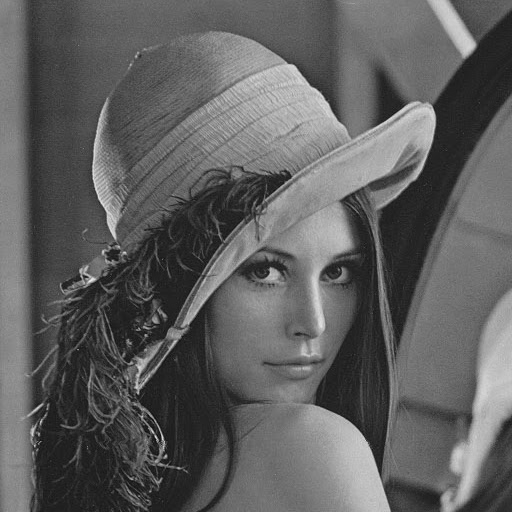
\includegraphics[width=4.5cm]{images/lenna.png}
				\caption{Original image}
				\label{subfig:org}
			\end{subfigure}
			~
			\begin{subfigure}[normla]{0.3\textwidth}
				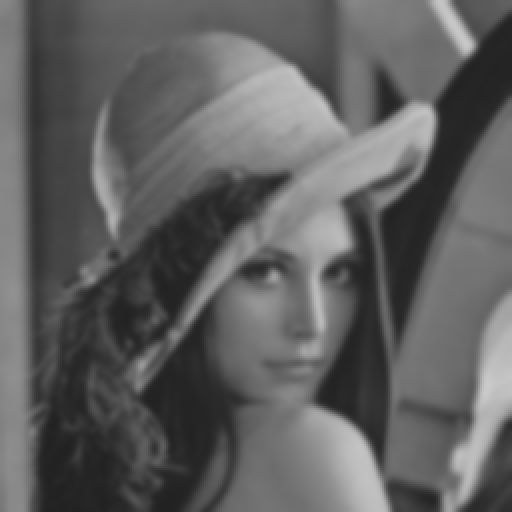
\includegraphics[width=4.5cm]{images/gaussian_at_sigma_3.png}
				\caption{Gaussian with $\sigma = 1.6$}
				\label{subfig:gauss1}
			\end{subfigure}
			~
			\begin{subfigure}[normla]{0.3\textwidth}
				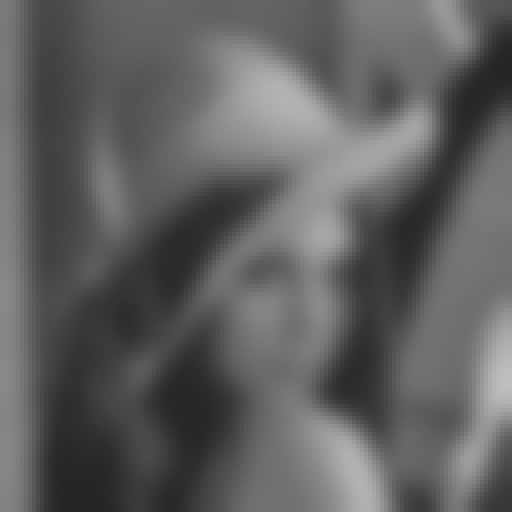
\includegraphics[width=4.5cm]{images/gaussian_at_sigma_10.png}
				\caption{Gaussian with $\sigma = ?$}
				\label{subfig:gauss2}
			\end{subfigure}
		
			\vspace{0.3cm}
		
			\begin{subfigure}[normla]{0.3\textwidth}
				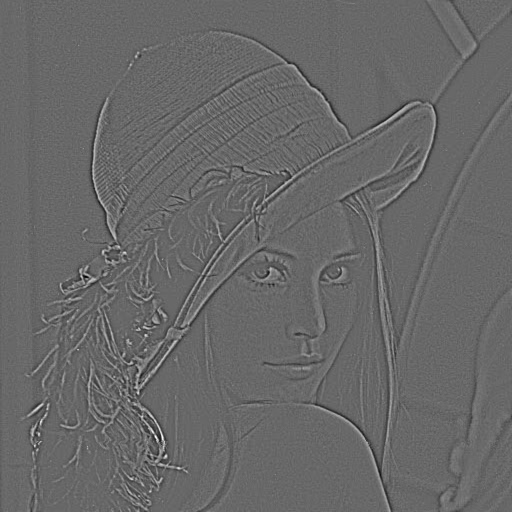
\includegraphics[width=4.5cm]{images/DoG_at_sigma_2.png}
				\caption{DoG with $\sigma_1$=1.6, $\sigma_2$=2.0}
				\label{subfig:org}
			\end{subfigure}
			~
			\begin{subfigure}[normla]{0.3\textwidth}
				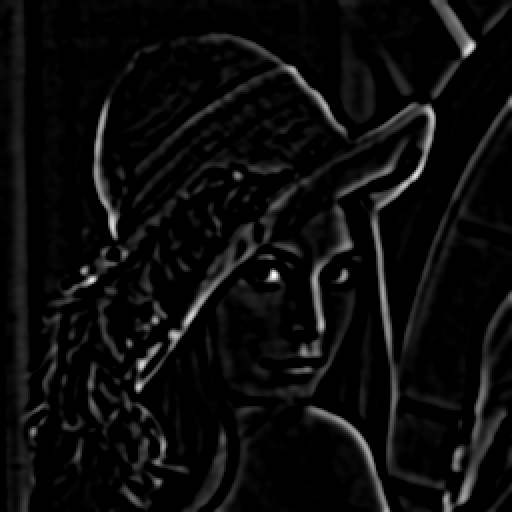
\includegraphics[width=4.5cm]{images/DoG_at_sigma_5.png}
				\caption{DoG with $\sigma_1$=?, $\sigma_2$=?}
				\label{subfig:org}
			\end{subfigure}
			~
			\begin{subfigure}[normla]{0.3\textwidth}		
				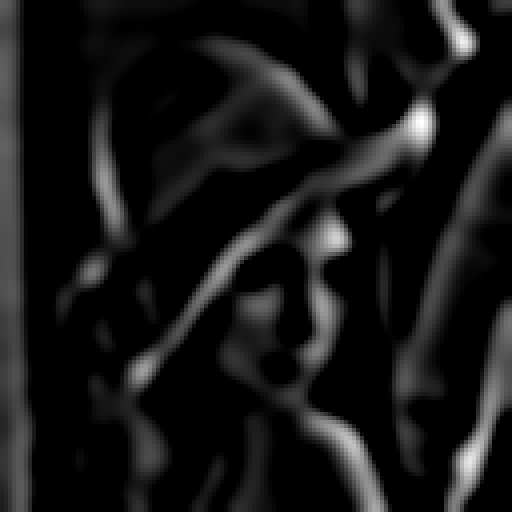
\includegraphics[width=4.5cm]{images/DoG_at_sigma_13.png}
				\caption{DoG with $\sigma_1$=?, $\sigma_2$=?}
				\label{subfig:org}
			\end{subfigure}
		\caption{This figure shows the impact of the Gaussian blur with different scales $\sigma$ on an image  as well as the difference of two neighboured Gaussian images.}
		\end{center}
	\end{figure}
	
	\subsection{Keypoint refinement}
	
	
	
	
	\subsection{Keypoint filtering}
	
	Some of the keypoints we obtained earlier might not represent good features due to a lack of contrast or unstable localization along an edge, so we need to reject such keypoints. 
	A low contrast also means that we might not find corresponding features of the same object in an image that has lightly been transformed from the original. Luckily, we can easily compute the contrast using the function from before (tayler expansion of the scale space function), but this time shifted by the exact location of the extremum. 
	
	$$
	D(\hat x) = D + 1/2 ...
	$$
	
	Lowe found that if the absolute value of that function is less than 0.03 there is just not enough contrast for it to be a stable feature. (normalized pixel values [0..1])
	
	Even if there is enough contrast the algorithm might still struggle to exactly localize a keypoint along an edge. That is why we rather have corner-like features than only edge-like.
	
	To further illustrate this problem, we can simply look at an arbitrary thick black line on white background as shown in Figure 3.x. Using the scale-space extrema we will find many potential keypoints all along this line, but their represented features will look all the same except for the two features at each end of the line. If you were given a patch of the middle section of that line, it would be impossible to tell the original location, whereas an end section can easily be matched by means of (its white part at the end)
	
	In order to mathematically determine whether a given feature is corner-like (/stable) or not, we can use a 2x2 Hessian matrix at its keypoint location and scale 
	
	\subsection{Orientation assignment}
	
	We have already shown that SIFT-Features are invariant to scale, but rotational invariance is just as important for numerus image processing tasks. For this purpose, Lowe assigns each keypoint one or more consistent orientations based on its neighborhood?s gradient directions and magnitudes.
	(define gradient)
	
	We want to use the most prominent gradient direction for each keypoint so that we achieve the same relative feature orientations on an image as its rotated counterpart.
	
	To find that most prominent gradient direction, each gradients magnitude in the keypoints neighborhood is added to the histogram bin with the closest gradient direction.  Even slight changes in 3D viewpoint can affect 
	That is the reason why the magnitude is weighted by a Gaussian function, so that gradients at the center of the keypoint have a higher impact than gradients further away.
	
	All gradient directions and magnitudes are precomputed using pixel differences for performance purposes [reference paper].
	
	
	\subsection{Constructing the feature descriptor}
	
	(define descriptor)

\end{document}
